\documentclass[11pt]{exam}
\usepackage[utf8]{inputenc}
\usepackage[a4paper,top=2cm,left=2cm,right=2cm,bottom=2cm]{geometry}
\usepackage{import}
\usepackage[T1]{fontenc}
\usepackage[german,ngerman]{babel}
\usepackage[table]{xcolor}
\usepackage{amsthm, esvect}
\usepackage{mathtools}
\RequirePackage{amssymb, amsfonts, amsmath, latexsym, verbatim, xspace}
\usepackage{systeme}
\usepackage{multicol}
\usepackage{multirow}
\usepackage{framed}
\usepackage{array}
\usepackage{ragged2e}
\usepackage{graphicx}
\usepackage{pdflscape}
\usepackage{epstopdf}
\usepackage{booktabs}
\usepackage{pdfpages}
\usepackage{float} % Allows putting an [H] in \begin{figure} to specify the exact location of the figure
\usepackage{wrapfig} % Allows in-line images such as the example fish picture
\usepackage{tikz, graphicx} % tikz
\usepackage[position=top]{subfig}
\usepackage[bookmarks=true]{hyperref}%Links
\usepackage{enumerate}
\usepackage{enumitem}
\usepackage[german,ruled,vlined,linesnumbered,algosection]{algorithm2e}
\usepackage[labelfont=sf]{caption}
\usepackage{lmodern}
\usepackage{lscape}
\usepackage{tabularx}
\usepackage{systeme}
\usepackage{hhline}
\usepackage{subfiles}
\usepackage{stackengine}
\usepackage{setspace}
\usepackage{MnSymbol}
\usepackage{tcolorbox}
\usepackage{bbm}
\usepackage{url}
\usepackage{xparse}
\usepackage{sectsty}
\usepackage{array}
\usepackage{ragged2e}
\usepackage{listings} %Stellt Code-Snippets sauber dar

% definiert die Sprache
\selectlanguage{German}

% add command for different dates in Swiss fashion
\newcommand{\monthwordlong}[1]{\ifcase#1 \or Januar\or Februar\or März\or April\or Mai\or Juni\or Juli\or August\or September\or Oktober\or November\or Dezember\fi}
\newcommand{\monthwordshort}[1]{\ifcase#1\or Jan\or Feb\or Mar\or Apr\or Mai\or Jun\or Jul\or Aug\or Sept\or Okt\or Nov\or Dez\fi}
\newcommand{\datelong}{\number\day.\:\monthwordlong{\the\month}\:\number\year}
\newcommand{\dateshort}{\number\day.\:\monthwordshort{\the\month}\:\number\year}

% define color of links inside a text
\definecolor{linkblue}{RGB}{0, 0, 80}
\definecolor{plotblue}{RGB}{100, 100, 255}
\definecolor{myblue}{RGB}{8,164,214}
\definecolor{myred}{RGB}{143,42,41}
\definecolor{forestgreen}{RGB}{34,139,34}
\definecolor{highdive}{RGB}{10,169,194}
\definecolor{charcoal}{RGB}{74,74,74}
\hypersetup{
	colorlinks=true,
	linkcolor=linkblue,
	filecolor=magenta,
	urlcolor=plotblue,
	citecolor=linkblue,
	pdfpagemode=FullScreen,
}


\lstdefinestyle{mystyle}{ % definiert den style des Code-Snippets
	%backgroundcolor=\color{backcolour},
	%commentstyle=\color{codegreen},
	%keywordstyle=\color{magenta},
	%numberstyle=\tiny\color{codegray},
	%stringstyle=\color{codepurple},
	basicstyle=\ttfamily\footnotesize,
	breakatwhitespace=false,
	breaklines=true,
	captionpos=b,
	keepspaces=true,
	%numbers=left,
	%numbersep=5pt,
	showspaces=false,
	showstringspaces=false,
	showtabs=false,
	tabsize=4
}
\lstset{style=mystyle}
\qformat{\Large\textbf{Aufgabe \thequestion\hfill\thepoints}}
\newlist{partes}{enumerate}{3}
\setlist[partes]{label=(\alph*)}
\newcommand{\parte}{\item}
\newlist{subpartes}{enumerate}{3}
\setlist[subpartes]{label=\roman*)}
\newcommand{\subparte}{\item}
\setlist[enumerate,1]{%(
	leftmargin=*, itemsep=12pt, label={\textbf{\arabic*.)}}}
\newcommand\answerbox{%%
	\fbox{\rule{2in}{0pt}\rule[-0.1ex]{0pt}{4ex}}}
\pointpoints{Punkt}{Punkte}
\hqword{Frage:}
\hpword{Mögliche Punkte:}
\hsword{Erreicht:}
\htword{Total}
\renewcommand*\half{.5}
\renewcommand{\solutiontitle}{\noindent\textbf{Lösung:}\par\noindent}

% Graphed boxes
\newcommand{\karos}[2]{
  \begin{tikzpicture}
    \draw[step=0.4cm,color=cyan,dotted] (0,0) grid (#1 cm ,#2 cm);
  %  \draw((#1)/2 cm,0)--((#1)/2 cm,/#2)/2cm)
  \end{tikzpicture}
}
\usetikzlibrary{arrows, petri, topaths, graphs}
\linespread{1.2} % Line spacing

%=========================================================
\newenvironment{parcols}[1][]{
    \begin{parts}\begin{multicols}{#1}
}{
    \end{multicols}\end{parts}
}
%=========================================================
\newenvironment{itemcols}[1][]{
	\begin{itemize}\begin{multicols}{#1}
		}{
	\end{multicols}\end{itemize}
}

%=========================================================
\newcommand{\antwort}[1]{
	{\setlength{\textwidth}{\textwidth}\fillwithgrid{#1cm}\vspace{5pt}}
}

%=========================================================
% Karriertes Papier für Antwort MIT OVERLAY
\tcbuselibrary{breakable,skins}
\usetikzlibrary{mindmap,trees}
\newlength\tindent
\setlength{\tindent}{\parindent}
\setlength{\parindent}{0pt}
\setlength{\parskip}{0pt}

\newtcolorbox{gridspace}[1]{%
	enhanced,
	breakable,
	blanker,
	boxrule=0pt,
	left=5mm,
	right=5mm,
	top=5.75mm,
	bottom=0mm,
	boxsep=0pt,
	height=#1cm,
	width=16cm,
	before upper={
		\begingroup
		\setlength{\baselineskip}{5.75mm}
		\setlength{\parskip}{0pt}
		\setlength{\lineskip}{0pt}
		% keep every paragraph on the grid rhythm
		%\everypar{\vspace{0pt}\strut}
		% math formulas shifted by one grid row
		\let\oldbracketopen\[
		\renewcommand{\[}{\vspace{-5mm}\oldbracketopen}
		% Align displayed formulas to the grid
		\setlength{\abovedisplayskip}{0pt}
		\setlength{\belowdisplayskip}{0pt}
		\setlength{\abovedisplayshortskip}{0pt}
		\setlength{\belowdisplayshortskip}{0pt}
		% Enumerate follows the same rhythm
		\setlist[enumerate]{leftmargin=6mm,itemsep=0mm,topsep=0pt,parsep=0pt,partopsep=0pt}
		\setlist[itemize]{leftmargin=6mm,itemsep=10mm,topsep=0pt,parsep=0pt,partopsep=0pt}},
	after upper={
		\endgroup},
	underlay={
		\draw[step=5mm,color=gray!55] (interior.south west) grid (interior.north east);}
}

\pagestyle{headandfoot}
\firstpageheader{}{}{\teacher}
\runningheader{}{}{\teacher}
\firstpagefooter{}{}{Seite \thepage\:von \numpages}
\runningfooter{}{}{Seite \thepage\:von \numpages}
%%
% Math Arrows
%%
\newcommand{\same}{\ensuremath{\Longleftrightarrow}}
\renewcommand{\to}{\ensuremath{\longrightarrow}}
\newcommand{\qsame}{\quad\same\quad}
\newcommand{\dsame}{\ensuremath{:\Leftrightarrow}}
\newcommand{\qdsame}{\quad\dsame\quad}
\newcommand{\ldsame}{\ensuremath{:\Longleftrightarrow}}
\newcommand{\samedef}{\ensuremath{\us {\text{def}} \Leftrightarrow}}
\newcommand{\qsamedef}{\quad\samedef\quad}
\newcommand{\lsamedef}{\ensuremath{\us {\text{def}} \Longleftrightarrow}}
\newcommand{\qlsamedef}{\quad\lsamedef\quad}


%%
% Mengendefinitionen
%%
\newcommand{\M}{\ensuremath{\mathcal{M}}}
\newcommand{\N}{\ensuremath{\mathbb{N}}}
\newcommand{\Z}{\ensuremath{\mathbb{Z}}}
\newcommand{\Q}{\ensuremath{\mathbb{Q}}}
\newcommand{\I}{\ensuremath{\mathbb{I}}}
\newcommand{\R}{\ensuremath{\mathbb{R}}}
\newcommand{\C}{\ensuremath{\mathbb{C}}}
\renewcommand{\S}{\ensuremath{\mathbb{S}}}
\newcommand{\Prim}{\ensuremath{\mathbb{P}}}
\newcommand{\0}{\ensuremath{\emptyset}}
\renewcommand{\Re}{\ensuremath{\operatorname{Re}}}
\renewcommand{\Im}{\ensuremath{\operatorname{Im}}}
\newcommand{\strich}{\ensuremath{\big\vert}}

%%
% Mengenoperation
%%
\renewcommand{\nin}{\not\in}


%%
% Logisches Und und Oder
%%
\newcommand{\sand}{\ensuremath{\; \land \;}}
\newcommand{\sor}{\ensuremath{\; \lor \;}}
\renewcommand{\*}{\ensuremath{\cdot}}
\newcommand{\oder}{\vee}
\newcommand{\n}{\neg}
\newcommand{\und}{\wedge}


%%
% Bei Integral, Summe,... die Grenzen über bzw.
% unter das Zeichen
%%
\renewcommand{\d}[1]{\ensuremath{\operatorname{d}\!{#1}}}
\newcommand{\Sum}{\sum\limits}
\newcommand{\Prod}{\prod\limits}
\newcommand{\Min}{\min\limits}
\newcommand{\Max}{\max\limits}
\newcommand{\Lim}{\lim\limits}
\newcommand{\Inf}{\inf\limits}
\newcommand{\Sup}{\sup\limits}
\newcommand{\Liminf}{\liminf\limits}
\newcommand{\Limsup}{\limsup\limits}
%\renewcommand{\Cup}{\bigcup\limits}
%\renewcommand{\Cap}{\bigcap\limits}
\newcommand{\Otimes}{\bigotimes\limits}
\newcommand{\Oplus}{\bigoplus\limits}


%%
% Arcus Cotangens, Logarithmus
%%
\let\oldsin\sin
\renewcommand{\sin}[1]{\oldsin{\left(#1\right)}}
\let\oldcos\cos
\renewcommand{\cos}[1]{\oldcos{\left(#1\right)}}
\let\oldtan\tan
\renewcommand{\tan}[1]{\oldtan{\left(#1\right)}}
\let\oldarcsin\arcsin
\renewcommand{\arcsin}[1]{\oldarcsin{\left(#1\right)}}
\let\oldarccos\arccos
\renewcommand{\arccos}[1]{\oldarccos{\left(#1\right)}}
\let\oldarctan\arctan
\renewcommand{\arctan}[1]{\oldarctan{\left(#1\right)}}
\let\oldln\ln
\renewcommand{\ln}[1]{\oldln{\left(#1\right)}}
\newcommand{\Log}[2]{\ensuremath{\operatorname{log}_{#1}\left(#2\right)}}
\newcommand{\e}{\operatorname{e}}
\renewcommand{\exp}[1]{\ensuremath{\operatorname{\e}^{#1}}}


%%
% Griechische Buchstaben
%%
\renewcommand{\epsilon}{\ensuremath{\varepsilon}}
\renewcommand{\phi}{\varphi}
\renewcommand{\l}{\lambda}
\renewcommand{\t}{\tau}


%%
% Bezeichnungen
%%
\newcommand{\Rgn}{\R_{>0}} % R grösser Null
\newcommand{\Rad}{\operatorname{Rad}}   % Radikal
\newcommand{\kgV}{\operatorname{kgV}}   % Kleinster gemeinsame Vielfache
\newcommand{\ggT}{\operatorname{ggT}}   % Grösster gemeinsame Teiler
\newcommand{\winkel}{\sphericalangle}          % Winkelsymbol
\DeclarePairedDelimiter\abs{\lvert}{\rvert} % besserer Betrag
\makeatletter
\let\oldabs\abs
\def\abs{\@ifstar{\oldabs}{\oldabs*}}
\makeatother


%%
% Vektorgeometrie
%%
\renewcommand{\v}[1]{\vv{#1}}       % besserer Pfeil über Buchstaben
\renewcommand{\vec}[2]{\begingroup\renewcommand{\arraystretch}{1}\left(\begin{array}{c} #1 \\ #2 \end{array}\right)\endgroup}   % two dimensional vector
\renewcommand{\Vec}[3]{\begingroup\renewcommand{\arraystretch}{1}\left(\begin{array}{c} #1 \\ #2 \\ #3 \end{array}\right)\endgroup}      % three dimensional vector


%%
% Text
%%
\newcommand*{\Ueq}[1]{\mathrel{\mathop{=}\limits_{\text{#1}}}}
\newcommand*{\Oeq}[1]{\mathrel{\stackrel{\text{#1}}{=}}}
\newcommand{\utext}[2]{\underbrace{#1}_{\substack{#2}}}
\newcommand{\otext}[2]{$\overbrace{\textrm{#1}}^{\textrm{#2}}$}
\newcommand{\lineortext}[1]{\hspace{0,1cm}\underline{\hspace{0.1cm}\hphantom{#1}\hspace{0.1cm}}\hspace{0,1cm}} % Lückentext erstellen
\newcommand{\gap}[1]{\rule{#1 cm}{1pt}}
%=========================================================
\newcommand{\theme}{Rationale Exponenten}
\newcommand{\teacher}{Jonas Guler}
%=========================================================
\begin{document}
\fontsize{14}{14}\selectfont
\begin{center}
    \huge\bf\theme
\end{center}

\begin{questions}
%=========================================================
%-----------------TESTFRAGEN - UMFORMUNGEN
%=========================================================
\noaddpoints
\question[\totalpoints]
\addpoints
\begin{parts}
	\part[2] Alice weiss noch nicht, was Potenzen der Art $5^{-2}$, $10^{-2}$ oder $3^{-16}$ genau bedeuten. Gib ihr eine gut nachvollziehbare Motivation für die Definition $a^{-n}:=\frac{1}{a^n}$ (für eine von 0 verschiedene reelle Basis a und eine natürliche Zahl n) an.
	\part[4] Verwandle den folgenden Term in ein klammer- und nennerfreies Produkt. Schreibe dabei bei jeder Umformung das entsprechende Gesetz dazu. \[\frac{a^5b^{-4}}{c^3d^{-2}}\*\frac{0.6c^{-5}d^4}{ab^{-2}}\]
\end{parts}


%---------------------------------------------------------
\question[6] % Barth K1.3 ÜA A2
Schreibe die folgenden Terme als eine einzige Potenz.
\begin{parcols}[3]
	\part $\displaystyle \frac{1}{x^6}\div\frac{1}{x^2}$ %i
	\part $\displaystyle \sqrt[10]{x}\*\left(\sqrt[4]{x}\div\sqrt[3]{x}\right)$ %p
	\part $\displaystyle \left(\sqrt[3]{x^2}\div\left(\sqrt{x}\right)^3\right)\*\frac{1}{\sqrt[6]{x}}$ %x
\end{parcols}


%---------------------------------------------------------
\question[4]
Ordne die Exponenten der folgenden Terme  der Grösse nach.
\begin{itemcols}[5]
	\item[\ ] $\displaystyle\left(\frac{1}{x}\right)^{-6}$
	\item[\ ] $\displaystyle\frac{1}{x^{2}}$
	\item[\ ] $\displaystyle\sqrt[4]{x^8}$
	\item[\ ] $\displaystyle\sqrt[4]{x}$
	\item[\ ] $\displaystyle\frac{1}{\sqrt[3]{x^9}}$
\end{itemcols}


%---------------------------------------------------------
\question[9]
Unten sind 3 Lösungswege angegeben. Erkläre, wo die Schülerin oder der Schüler einen Fehler gemacht hat und löse die Aufgabe korrekt. (Im Resultat dürfen keine negativen Exponenten vorkommen.)
\begin{parts}
    \part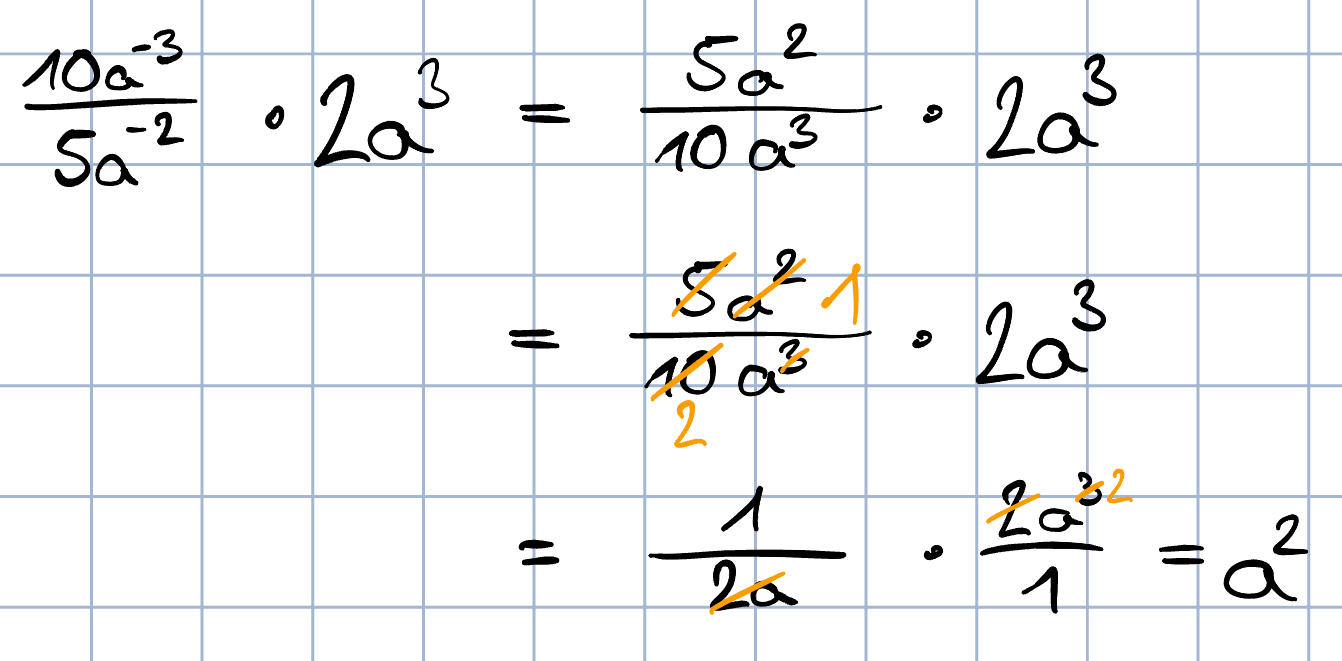
\includegraphics[scale=0.2]{data-algebra/5a.png}
    \part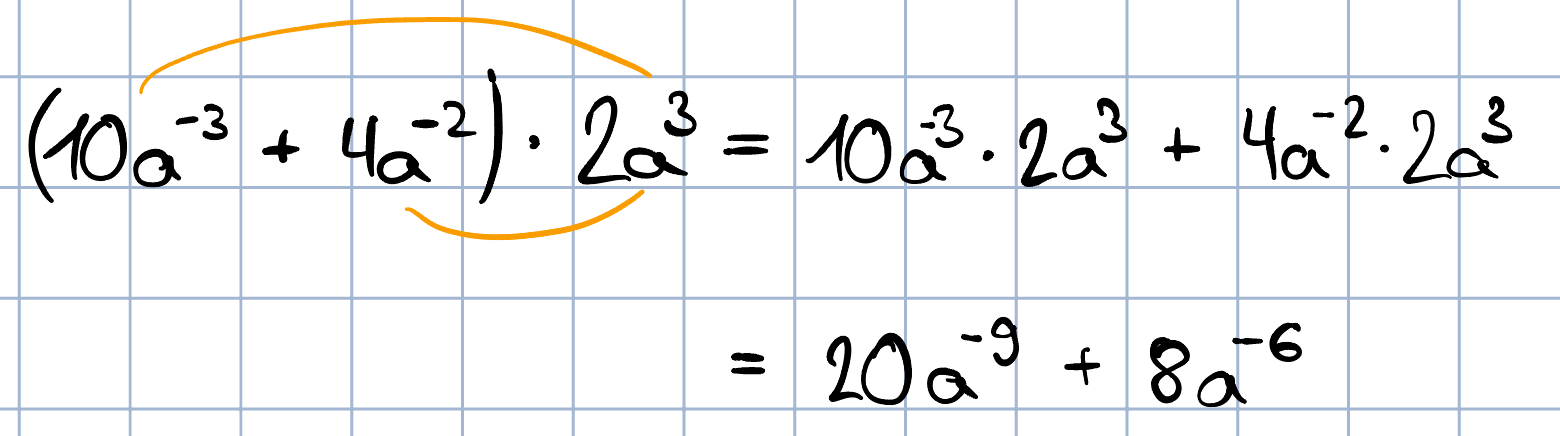
\includegraphics[scale=0.25]{data-algebra/5b.png}
    \part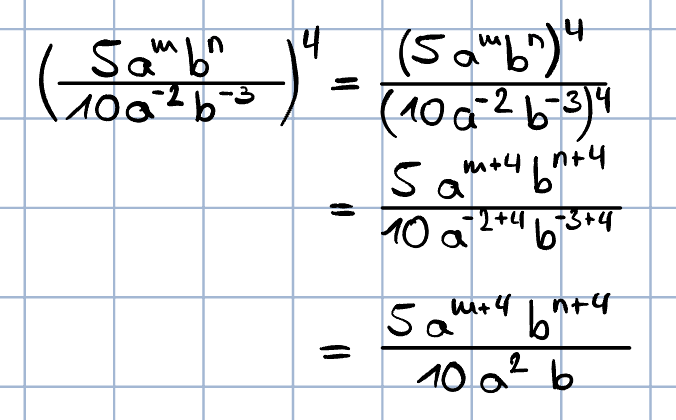
\includegraphics[scale=0.3]{data-algebra/5d.png}
\end{parts}


%---------------------------------------------------------
\question[9] %
Unten sind 3 Lösungswege angegeben. Erkläre, wo die Schülerin oder der Schüler einen Fehler gemacht hat und löse die Aufgabe korrekt. (Im Resultat dürfen keine negativen Exponenten vorkommen.)
\begin{parts}
    \part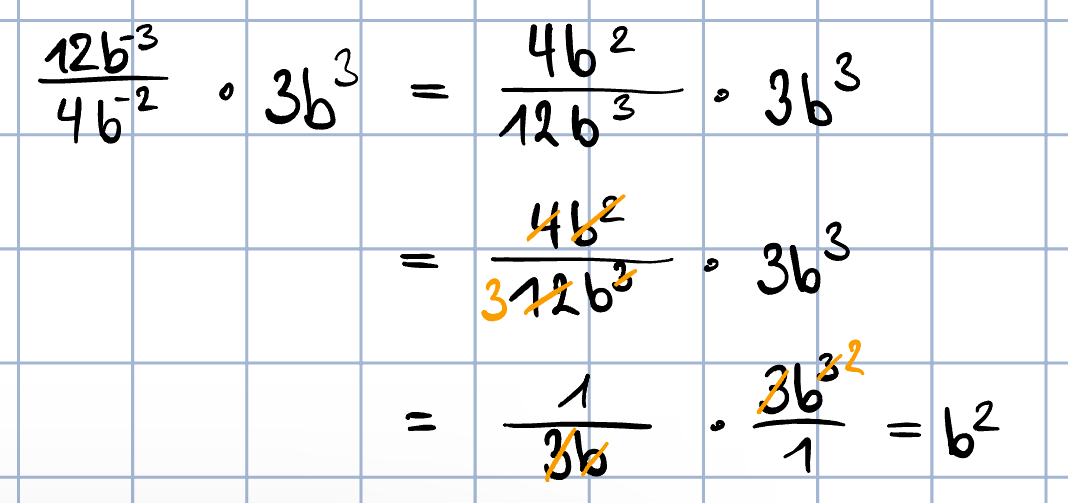
\includegraphics[scale=0.2]{data-algebra/5a-rep.png}
    \part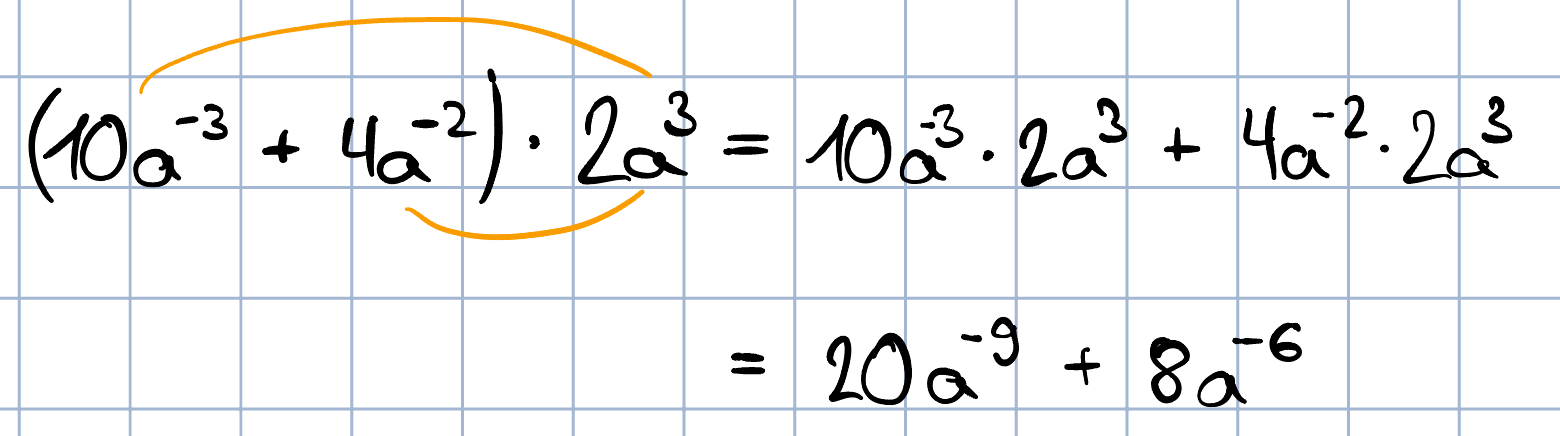
\includegraphics[scale=0.25]{data-algebra/5b.png}
    \part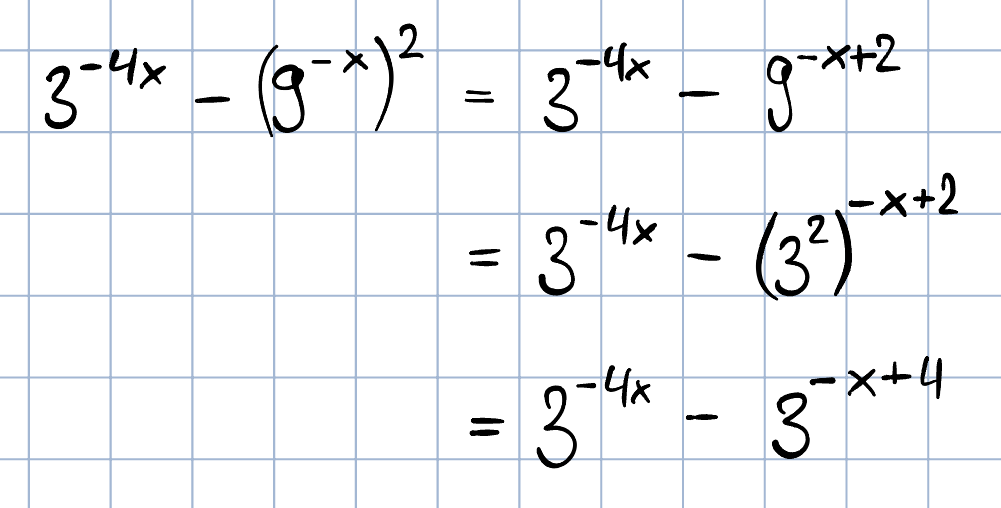
\includegraphics[scale=0.3]{data-algebra/5c.png}
\end{parts}


%---------------------------------------------------------
\question[4] %
Bestimme die fehlenden Exponenten $\triangle$ oder die fehlende Basis $\square$.
\begin{parts}
    \part $6^{12}\cdot6^\triangle=6^{-3}$
    \part $5^8\cdot5^\triangle=5^3$
    \part $2^\triangle=8^{-4}$
    \part $\square^6=16^3$
\end{parts}


%---------------------------------------------------------
\question[4] %
Bestimme die fehlenden Exponenten $\triangle$ oder die fehlende Basis $\square$.
\begin{parts}
    \part $6^{2}:6^\triangle=6^{-m+2}$
    \part $5^{-6}\cdot5^\triangle=5^4$
    \part $2^\triangle=8^{-4}$
    \part $\square^6=16^3$
\end{parts}


%---------------------------------------------------------
\question[2]
Entscheide in der Tabelle unten, ob die Aussagen wahr oder falsch sind. Die Antworten müssen nicht begründet werden.\newline
\begin{small}
	Bewertung: Für $0-2$ korrekte Antworten gibt es keine Punkte; $3$ korrekte Antworten $1$ Punkt und falls alle Antworten korrekt sind, gibt es $2$ Punkte.
\end{small}
\begingroup
\renewcommand{\arraystretch}{1.5}
\begin{table}[H]
	\centering
	\begin{tabular}{|p{12cm}|c|c|}\hline
		& wahr & falsch \\\hline
		Falls $a\neq0$ gilt, dann ist folgende Umformung korrekt  $a^{-3}+a^{-3}+a^{-3}=a^{-2}$. & & \\\hline
		$\displaystyle 9^{\frac{3}{2}}\in\N$ & & \\\hline
		Falls $a\neq0$ gilt, dann ist folgende Umformung korrekt  $\displaystyle \left(a^2\right)^2=a^{\left(2^2\right)}$. & & \\\hline
		Falls $a\neq0$ gilt, dann ist folgende Umformung korrekt  $2^{-3}\*(-2)^3=1$. & & \\\hline
	\end{tabular}
\end{table}
\endgroup


%=========================================================
%-----------------TESTFRAGEN - POTENZFUNKTIONEN
%=========================================================
\newpage
\question[5] % Potenzfunktionen
\begin{minipage}{0.6\linewidth}
	Zwei Potenzfunktionen der Form $f:y=a\*x^p$ sind im Graphen auf der rechten Seite abgebildet.
	\begin{parts}
		\part Gib die Funktionsgleichung der beiden skizzierten Potenzfunktionen an. Treffe dazu sinnvolle Annahmen für die Koordinaten der grau markierten Punkte. Du darfst nur diese Punkte verwenden.
		\part Spiegle den \textcolor{plotblue}{blauen} Funktionsgraphen an der $x-$Achse. Gib die Funktionsgleichung sowie Definitions- und Wertemenge des gespiegelten Funktionsgraphen an.
	\end{parts}
\end{minipage}
\hfill
\begin{minipage}{0.375\linewidth}
	\centering
	\begin{tikzpicture}[cross/.style={draw, cross out, minimum size=2*(#1-1pt), inner sep=0pt, outer sep=0pt}, x=10mm, y=10mm,
		>=latex,   %Voreinstellung für Pfeilspitzen
		font= \footnotesize, scale=0.7]
		%Raster zeichnen
		\draw [color=gray!50]  [step=10mm] (-4.3,-2.3) grid (4.3,8.3);
		% Achsen zeichnen
		\draw[->,thick] (-4.3,0) -- (4.8,0) node[right, below] {\normalsize $x$};
		\draw[->,thick] (0,-2.3) -- (0,8.8) node[above, left] {\normalsize $y$};
		% Achsen beschriften
		\foreach \x in {-4,...,-2,-1,1,2,...,4} \draw (\x,-.1) -- (\x,.1) node[below=4pt] {$\x$};
		\foreach \y in {-2,-1,1,2,...,8} \draw (-.1,\y) -- (.1,\y) node[left=4pt] {$\y$};
		% Besserer Ursprung
		\draw[color=black] (0pt,-7pt) node[right] {$0$};
		%Funktionen zeichnen:
		\clip(-4.3,-2.3) rectangle (4.3,8.3); %Bildbereich
		\draw[plotblue,thick,domain=-4.3:-0.5,samples=100] plot (\x, {8/(\x)^3});
		\draw[plotblue,thick,domain=0.5:4.3,samples=100] plot (\x, {8/(\x)^3});
		\draw[forestgreen,thick,domain=-3:3,samples=200] plot (\x, {0.25*(\x)^4});
		%Beschriftung
		\draw[fill=black!40] (1,8) circle (3pt);
		\draw[fill=black!40] (-2,-1) circle (3pt);
		\draw[fill=black!40] (0,0) circle (3pt);
		\draw[fill=black!40] (2,4) circle (3pt);
	\end{tikzpicture}
\end{minipage}



%---------------------------------------------------------
\question[5] %
Gegeben seien die folgenden vier Funktionsgleichungen der Funktionen $f_1,f_2,f_3$ und $f_4$ und ihre entsprechende Graphen. Die eingezeichneten Punkte haben ganzzahlige Koordinaten.
\begin{parts}
	\part Fülle die Nummer des richtigen Graphen ins entsprechende Kästchen ein.
	\part Von einem Graphen fehlt die Funktionsgleichung. Wie lautet sie?
\end{parts}
\begingroup
\renewcommand{\arraystretch}{1.5}
\begin{table}[H]
	\centering
	\begin{tabular}{|c|c|c|c|c|}\hline
		Funktionsgleichung: & $y=f_1(x)=x^3$ & $y=f_2(x)=\sqrt{2x-2}$ & $y=f_3(x)=x^2+2x$ & $y=f_4(x)=\frac{1}{x^4-2}$ \\\hline
		Graph Nummer: & & & & \\\hline
	\end{tabular}
\end{table}
\endgroup
\begin{table}[H]
	\centering
	\begin{tabular}{|c|c|c|}\hline
		1. \newline
		\begin{tikzpicture}[cross/.style={draw, cross out, minimum size=2*(#1-1pt), inner sep=0pt, outer sep=0pt}, x=10mm, y=10mm,
			>=latex,   %Voreinstellung für Pfeilspitzen
			font= \footnotesize, scale=0.7]
			%Raster zeichnen
			\draw [color=gray!50]  [step=10mm] (-3.3,-1.3) grid (1.3,3.3);
			% Achsen zeichnen
			\draw[->,thick] (-3.3,0) -- (1.8,0) node[right, below] {\normalsize $x$};
			\draw[->,thick] (0,-1.3) -- (0,3.8) node[above, left] {\normalsize $y$};
			% Achsen beschriften
			\foreach \x in {-3,-2,-1,1} \draw (\x,-.1) -- (\x,.1) node[below=4pt] {$\x$};
			\foreach \y in {-1,1,2,3} \draw (-.1,\y) -- (.1,\y) node[left=4pt] {$\y$};
			% Besserer Ursprung
			\draw[color=black] (0pt,-10pt) node[right] {$0$};
			%Funktionen zeichnen:
			\clip(-3.3,-1.3) rectangle (2.3,3.3); %Bildbereich
			\draw[plotblue,thick,domain=-3.3:2.3,samples=100] plot (\x, {(\x)^2+2*\x});
			%Beschriftung
			\draw[fill=black!40] (-1,-1) circle (3pt);
			\draw[fill=black!40] (-3,3) circle (3pt);
			\draw[fill=black!40] (0,0) circle (3pt);
		\end{tikzpicture} &
		2. \newline
		\begin{tikzpicture}[cross/.style={draw, cross out, minimum size=2*(#1-1pt), inner sep=0pt, outer sep=0pt}, x=10mm, y=10mm,
			>=latex,   %Voreinstellung für Pfeilspitzen
			font= \footnotesize, scale=0.6]
			%Raster zeichnen
			\draw [color=gray!50]  [step=10mm] (-2.3,-2.3) grid (4.3,3.3);
			% Achsen zeichnen
			\draw[->,thick] (-2.3,0) -- (4.8,0) node[right, below] {\normalsize $x$};
			\draw[->,thick] (0,-2.3) -- (0,3.8) node[above, left] {\normalsize $y$};
			% Achsen beschriften
			\foreach \x in {-2,-1,1,2,...,4} \draw (\x,-.1) -- (\x,.1) node[below=4pt] {$\x$};
			\foreach \y in {-2,-1,1,2,3} \draw (-.1,\y) -- (.1,\y) node[left=4pt] {$\y$};
			% Besserer Ursprung
			\draw[color=black] (0pt,-7pt) node[right] {$0$};
			%Funktionen zeichnen:
			\clip(-2.3,-2.3) rectangle (4.3,3.3); %Bildbereich
			\draw[plotblue,thick,domain=-2.3:-0.5,samples=100] plot (\x, {1/(\x)^4-2});
			\draw[plotblue,thick,domain=0.5:4.3,samples=100] plot (\x, {1/(\x)^4-2});
			%Beschriftung
			\draw[fill=black!40] (-1,-1) circle (3pt);
			\draw[fill=black!40] (1,-1) circle (3pt);
		\end{tikzpicture} &
		3. \newline
		\begin{tikzpicture}[cross/.style={draw, cross out, minimum size=2*(#1-1pt), inner sep=0pt, outer sep=0pt}, x=10mm, y=10mm,
			>=latex,   %Voreinstellung für Pfeilspitzen
			font= \footnotesize, scale=0.6]
			%Raster zeichnen
			\draw [color=gray!50]  [step=10mm] (-2.3,-2.3) grid (3.3,3.3);
			% Achsen zeichnen
			\draw[->,thick] (-2.3,0) -- (3.8,0) node[right, below] {\normalsize $x$};
			\draw[->,thick] (0,-2.3) -- (0,3.8) node[above, left] {\normalsize $y$};
			% Achsen beschriften
			\foreach \x in {,-2,-1,1,2,...,3} \draw (\x,-.1) -- (\x,.1) node[below=4pt] {$\x$};
			\foreach \y in {-2,-1,1,2,...,3} \draw (-.1,\y) -- (.1,\y) node[left=4pt] {$\y$};
			% Besserer Ursprung
			\draw[color=black] (0pt,-7pt) node[right] {$0$};
			%Funktionen zeichnen:
			\clip(-2.3,-2.3) rectangle (2.3,3.3); %Bildbereich
			\draw[plotblue,thick,domain=-2:2,samples=100] plot (\x, {(\x^3)});
			%Beschriftung
			\draw[fill=black!40] (-1,-1) circle (3pt);
			\draw[fill=black!40] (1,1) circle (3pt);
			\draw[fill=black!40] (0,0) circle (3pt);
		\end{tikzpicture} \\\hline
	\end{tabular}
\end{table}
\begin{table}[H]
	\centering
	\begin{tabular}{|c|c|}\hline
		4. \newline
		\begin{tikzpicture}[cross/.style={draw, cross out, minimum size=2*(#1-1pt), inner sep=0pt, outer sep=0pt}, x=10mm, y=10mm,
			>=latex,   %Voreinstellung für Pfeilspitzen
			font= \footnotesize, scale=0.7]
			%Raster zeichnen
			\draw [color=gray!50]  [step=10mm] (-0.3,-1.3) grid (9.3,4.3);
			% Achsen zeichnen
			\draw[->,thick] (-0.3,0) -- (9.8,0) node[right, below] {\normalsize $x$};
			\draw[->,thick] (0,-1.3) -- (0,4.8) node[above, left] {\normalsize $y$};
			% Achsen beschriften
			\foreach \x in {1,2,...,9} \draw (\x,-.1) -- (\x,.1) node[below=4pt] {$\x$};
			\foreach \y in {-1,1,2,...,4} \draw (-.1,\y) -- (.1,\y) node[left=4pt] {$\y$};
			% Besserer Ursprung
			\draw[color=black] (0pt,-10pt) node[right] {$0$};
			%Funktionen zeichnen:
			\clip(-0.3,-1.3) rectangle (9.3,4.3); %Bildbereich
			\draw[plotblue,thick,domain=1:9.3,samples=100] plot (\x, {(2*(\x)-2)^(1/2)});
			%Beschriftung
			\draw[fill=black!40] (3,2) circle (3pt);
			\draw[fill=black!40] (9,4) circle (3pt);
		\end{tikzpicture} &
		5. \newline
		\begin{tikzpicture}[cross/.style={draw, cross out, minimum size=2*(#1-1pt), inner sep=0pt, outer sep=0pt}, x=10mm, y=10mm,
			>=latex,   %Voreinstellung für Pfeilspitzen
			font= \footnotesize, scale=0.6]
			%Raster zeichnen
			\draw [color=gray!50]  [step=10mm] (-3.3,-3.3) grid (4.3,3.3);
			% Achsen zeichnen
			\draw[->,thick] (-3.3,0) -- (4.8,0) node[right, below] {\normalsize $x$};
			\draw[->,thick] (0,-3.3) -- (0,3.8) node[above, left] {\normalsize $y$};
			% Achsen beschriften
			\foreach \x in {-3,-2,-1,1,2,...,4} \draw (\x,-.1) -- (\x,.1) node[below=4pt] {$\x$};
			\foreach \y in {-3,-2,-1,1,2,3} \draw (-.1,\y) -- (.1,\y) node[left=4pt] {$\y$};
			% Besserer Ursprung
			\draw[color=black] (0pt,-7pt) node[right] {$0$};
			%Funktionen zeichnen:
			\clip(-3.3,-3.3) rectangle (4.3,3.3); %Bildbereich
			\draw[plotblue,thick,domain=-3.3:-0.5,samples=100] plot (\x, {2/(\x)^5});
			\draw[plotblue,thick,domain=0.5:4.3,samples=100] plot (\x, {2/(\x)^5});
			%Beschriftung
			\draw[fill=black!40] (-1,-2) circle (3pt);
			\draw[fill=black!40] (1,2) circle (3pt);
		\end{tikzpicture} \\\hline
	\end{tabular}
\end{table}

\end{questions}
\end{document}